\chapter{A deep-learning approach for inference of selective sweeps from the ancestral recombination graph}

\textit{Content of this chapter was previously uploaded to bioRxiv (2021) under the title "SIA: Selection Inference Using the Ancestral Recombination Graph" by Hussein A. Hejase, Ziyi Mo, Leonardo Campagna and Adam Siepel. The manuscript was published in Molecular Biology and Evolution (2021) under the title "A Deep-Learning Approach for Inference of Selective Sweeps from the Ancestral Recombination Graph". H.H. and Z.M. contributed equally to this work.}

\section{Abstract}

Detecting signals of selection from genomic data is a central problem in population genetics. Coupling the rich information in the ancestral recombination graph (ARG) with a powerful and scalable deep-learning framework, we developed a novel method to detect and quantify positive selection: \textbf{S}election \textbf{I}nference using the \textbf{A}ncestral recombination graph (SIA). Built on a Long Short-Term Memory (LSTM) architecture, a particular type of a Recurrent Neural Network (RNN), SIA can be trained to explicitly infer a full range of selection coefficients, as well as the allele frequency trajectory and time of selection onset. We benchmarked SIA extensively on simulations under a European human demographic model, and found that it performs as well or better as some of the best available methods, including state-of-the-art machine-learning and ARG-based methods. In addition, we used SIA to estimate selection coefficients at several loci associated with human phenotypes of interest. SIA detected novel signals of selection particular to the European (CEU) population at the \textit{MC1R} and \textit{ABCC11} loci. In addition, it recapitulated signals of selection at the \textit{LCT} locus and several pigmentation-related genes. Finally, we reanalyzed polymorphism data of a collection of recently radiated southern capuchino seedeater taxa in the genus \textit{Sporophila} to quantify the strength of selection and improved the power of our previous methods to detect partial soft sweeps. Overall, SIA uses deep learning to leverage the ARG and thereby provides new insight into how selective sweeps shape genomic diversity.

\section{Introduction}

The ability to accurately detect and quantify the influence of selection from genomic sequence data enables a wide variety of insights, ranging from understanding historical evolutionary events to characterizing the functional and disease relevance of observed or potential genetic variants. Adaptive evolution is driven by increases in frequency of alleles that enhance reproductive fitness. In addition, alleles experiencing such positive selection often provide insights into the functional or mechanistic basis of phenotypes of interest. Examples of genetic determinants of important phenotypic traits under selection in human populations include a family of mutations in the hemoglobin-$\beta$ cluster, which confer resistance to malaria and are at high frequencies in many populations (\cite{currat_molecular_2002,ohashi_extended_2004}), loci controlling growth factor signaling pathways that contribute to short stature in Western Central African hunter-gatherer populations (\cite{jarvis_patterns_2012,lachance_evolutionary_2012}), as well as mutations in several genes involved in immunity, hair follicle development, and skin pigmentation (\cite{sabeti_genome-wide_2007})(reviewed in \cite{sabeti_positive_2006, kelley_positive_2008,fu_selection_2013,hejase_summary_2020}).

Population genetic methods predominantly identify positive selection throu\-gh the detection of selective sweeps. As the frequency of an advantageous allele increases, linked variants in the vicinity can “hitchhike” to high frequency, leading to local reductions in genetic diversity. Previous approaches to detecting selective sweeps (such as traditional summary statistics [\cite{tajima_statistical_1989}], approximate likelihood and Approximate Bayesian Computation [ABC] methods [\cite{peter_distinguishing_2012}], or supervised machine-learning [ML] methods [\cite{schrider_shic_2016, kern_diploshic_2018}]) exploit the effect of genetic hitchhiking on the spatial haplotype structure and site frequency spectrum (SFS). Summary statistics have the advantage of being fast and easy to compute, but may confound the effects of selection on genetic diversity with the effects of complex demographic histories including bottlenecks, population expansions, and structured populations. Besides, they cannot easily be used to estimate the value of the selection coefficient. Approximate likelihood and ABC methods, on the other hand, can provide an estimate of the strength of selection by aggregating multiple summary statistics (\cite{peter_distinguishing_2012}), but can be prohibitively computationally expensive when applied at a large scale. ML methods for inferring selection can be more scalable and can capture complex nonlinear relationships among features. With the exception of a handful of recently developed methods that operate on the multiple sequence alignment itself (\cite{flagel_unreasonable_2019,torada_imagene_2019}), however, the majority of ML approaches to selection inference solely make use of traditional summary statistics as features for prediction. In short, previous methods (including ABC and most ML methods) predominantly rely on low-dimensional summary statistics, which, even in combination, capture only a small portion of the information in the sequence data.

Recently, a new generation of inference methods have made it possible to go beyond summary statistics and estimate or sample a full ancestral recombination graph (ARG) (\cite{hudson_gene_1990,griffiths_ancestral_1996,wiuf_recombination_1999}) for a collection of sequences of interest. The ARG is a complex data structure that summarizes the shared evolutionary history and recombination events that have occurred in a collection of DNA sequences, and therefore contains highly informative features that can potentially be leveraged to make accurate inferences about selection. The ARG representation is interchangeable with a sequence of local genealogies along the genome and the recombination events that transform each genealogy to the next. The influence of selection on each allele can be characterized from the ARG, based on departures from the patterns of coalescence and recombination expected under neutrality as reflected in the local genealogies. Traditional ARG inference methods (\cite{hein_heuristic_1993,song_constructing_2005,minichiello_mapping_2006,kuhner_lamarc_2006,ofallon_acg_2013}) were restricted in accuracy and scalability, limiting the practical application of ARGs. Recent advances (\cite{rasmussen_genome-wide_2014}), however, have enabled scalable yet statistically rigorous genome-wide ARG inference with dozens of genomes. Moreover, methods such as Relate (\cite{speidel_method_2019}) and tsinfer (\cite{kelleher_inferring_2019}) have further dramatically improved the scalability of ARG inference to accommodate thousands or even hundreds of thousands of genomes. The latest progress in genealogical inference has paved the way for ARG-based methods to address many different questions in population genetics (\cite{arenas_importance_2013,rasmussen_genome-wide_2014,kelleher_inferring_2019,speidel_method_2019}).

One natural way to exploit the richness of the ARG representation in inference of selection would be to extract features from inferred ARGs and feed them into a modern supervised ML framework. Deep-learning methods, in particular, have recently achieved unprecedented success on a variety of challenging problems, including image recognition, machine translation, and game-play (\cite{lecun_deep_2015}). Deep learning is also highly flexible, providing many opportunities for the design of novel model architectures motivated by biological knowledge. An ARG-guided deep-learning model could potentially provide new insight into how natural selection impacts the human genome, human diseases and other phenotypes, and human evolution.

With these goals in mind, we developed a new method, called SIA (\textbf{S}election \textbf{I}nference using the \textbf{A}ncestral recombination graph), that uses a Recurrent Neural Network (RNN) (\cite{hochreiter_long_1997,maas_learning_2011}) to infer the selection coefficient and allele frequency (AF) trajectory of a variant that maps to a gene tree embedded in an ARG. Rather than relying on traditional sequence-based summary statistics, SIA makes use of features based on the local genealogies extracted from the ARG. Based on these local topological features, SIA learns to infer the selection coefficient and AF trajectory of a beneficial variant (see Fig. \ref{fig:SIA-F1}). As described below, SIA performs well on benchmarks and is reasonably robust to model mis-specification. Applying SIA to data from the 1000 Genomes Northern and Western European (CEU) population, we identified new and known loci under positive selection that are associated with a variety of phenotypes and estimated selection coefficients at these loci. In addition, using SIA, we built on our previous work (\cite{hejase_genomic_2020}) on a bird species-complex in the genus Sporophila by elucidating the strength and targets of selection at specific loci tied to a collection of rapid speciation events. Overall, SIA is the first method that couples ARG-based features with an ML approach for population genetic inference.

\begin{figure}[h]
    \centering
    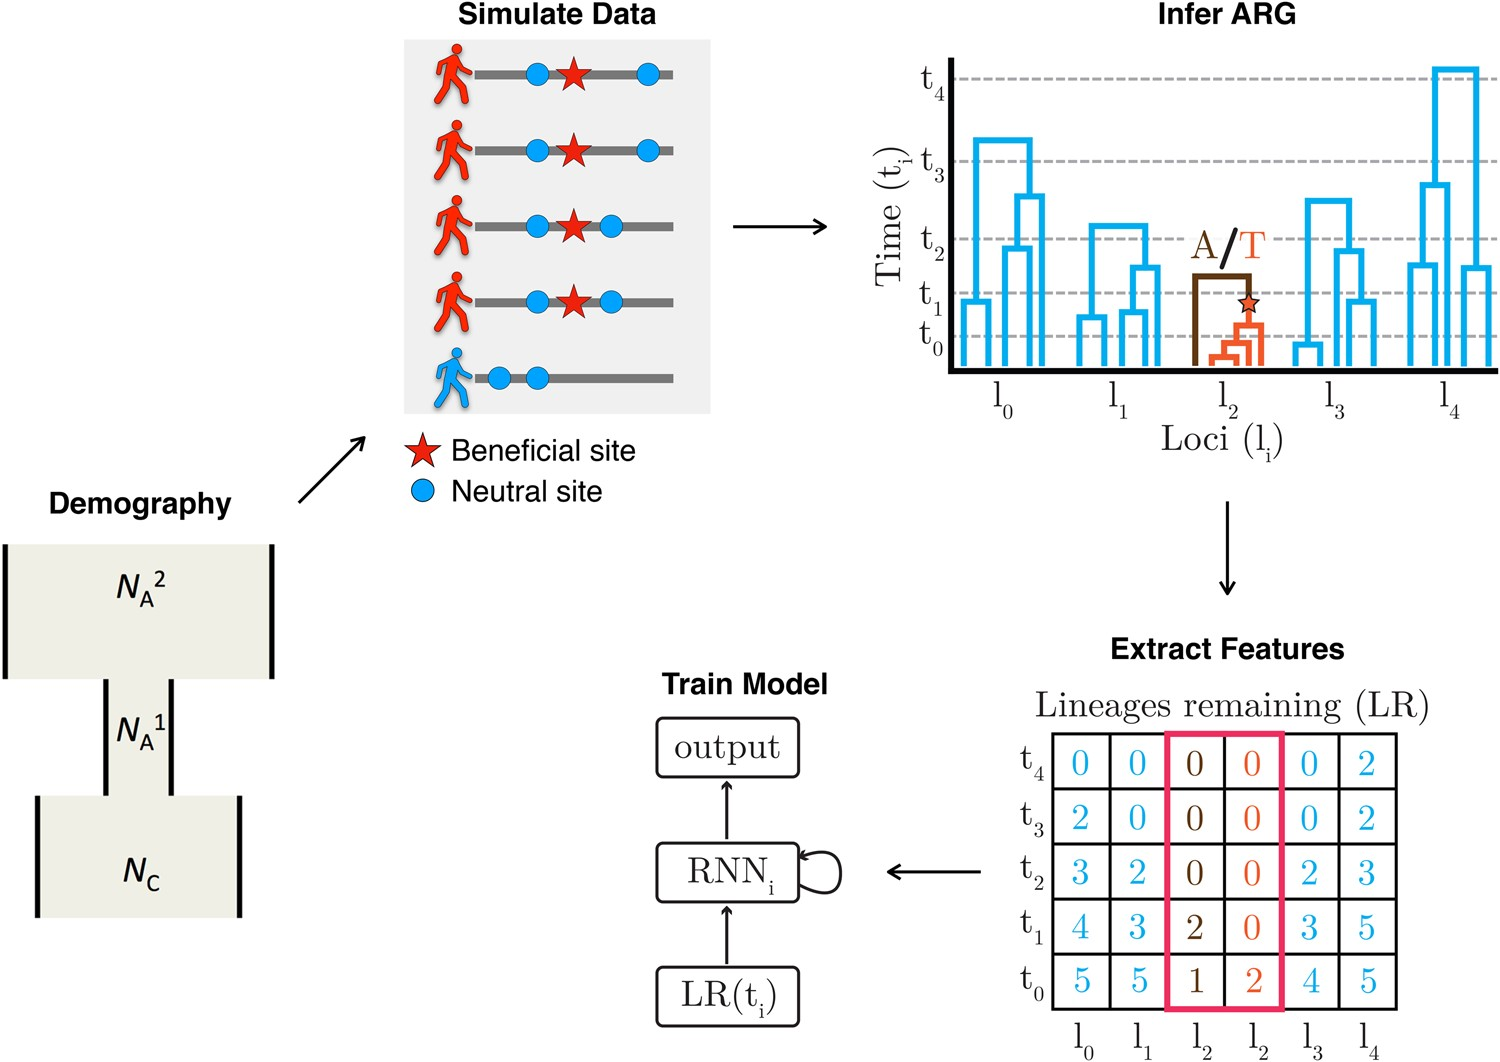
\includegraphics[width=\textwidth]{SIA_figs/SIA_F1.jpeg}
    \caption[A high-level framework for automating the detection of selective sweeps.]{\textbf{A high-level framework for automating the detection of selective sweeps.} We first estimate the demographic history for the population of interest, then based on the estimated demographic history, we simulate neutral regions and sweeps using the discoal simulator (\cite{kern_discoal_2016}). We proceed with ARG inference and then extract ARG-level statistics from each simulated region. The ARG-level statistics are used as features for a deep-learning RNN model. Finally, the trained model is applied to the empirical data to infer sweeps, selection coefficients, and AF trajectories.}
    \label{fig:SIA-F1}
\end{figure}

\section{Results}
\subsection{Methodological Overview}
SIA is based on an RNN that is trained to predict selection at a genomic site from genealogical features at that site of interest and nearby sites (see \nameref{methods} for detailed descriptions; see Fig. \ref{fig:SIA-F1} for a conceptual overview of SIA; and Fig. \href{https://academic.oup.com/mbe/article/39/1/msab332/6433161#supplementary-data}{S1} online for an illustration of ARG features and the RNN architecture). Based on the demography of a particular population of interest, training data including genomic regions under various strengths of selection are simulated. The ARG is then inferred from each simulated data set. ARG-level statistics are extracted at the site under selection (or a neutral site) as features to be used as input to the deep-learning model. Specifically, we use lineage counts at a set of discrete time points as a fixed-dimension encoding of a genealogy. The encoding of the genealogy at the focal site as well as similar encodings of flanking genealogies constitute the feature vector for that site. SIA uses a Long Short-Term Memory (LSTM) architecture, designed specifically to handle the temporal nature of the feature set. The LSTM unrolls temporally such that the lineage counts at each time point are fed to the network iteratively. Finally, the model trained on simulations is applied to ARGs inferred from empirical data to identify sweeps, infer selection coefficients, and AF trajectories.

\subsection{Classification of Sweeps}



\section{Discussion}

\section{Materials and Methods} \label{methods}

\section{Supplementary Material}

Supplementaty figures are available at \href{https://academic.oup.com/mbe/article/39/1/msab332/6433161#supplementary-data}{\textit{Molecular Biology and Evolution} online}. The simulation scripts and code for building and training the SIA model are publicly available on \href{https://github.com/CshlSiepelLab/arg-selection}{GitHub}.